\chapter{Conoscenze di base} 
In questo capitolo verranno esplorate le conoscenze fondamentali che costituiscono il punto di partenza teorico per lo sviluppo del progetto. Queste conoscenze sono
 essenziali per comprendere appieno il contesto e i concetti chiave che saranno discussi
 nei prossimi capitoli.
 
\section{ROS2 - Robotic Operating System}
ROS2 è un middleware basato su un meccanismo di publisher e subscriber che per
mette l’interazione, attraverso lo scambio di informazioni, tra diversi processi ROS.\\
Il progetto è stato sviluppato all'interno di un workframe ROS2 (ROS Foxy)\cite{doi:10.1126/scirobotics.abm6074} instroduciamo quindi alcuni componenti della sua terminologia fondamentale \cite{rosDocumentation}: \\
\begin{enumerate}
\item \textbf{ROS graph}: Si riferisce ad una rappresentazione visuale o concettuale della rete
 di comunicazione e delle interconnesioni tra i nodi all’interno di ROS. Questa
 rappresentazione grafica mostra come i nodi comunicano tra loro, inviando e
 ricevendo messaggi tramite i topic e come sono collegati all’interno di ROS.
\item \textbf{ROS topic}: I topic vengono utilizzati come canali di comunicazione tra diversi processi, in modo da scambiarsi dati attraverso dei messaggi.
\item \textbf{ROS nodes}:  I nodi possono essere visualizzati come unità di elaborazione,
 ovvero sono quelle entità che si devono scambiare dati fra di loro, questo avviene tramite i publisher o subscriber, infatti i nodi hanno la capacità di:\\
 
\begin{itemize}

\item \textbf{Sottoscriversi} ad un topic e quindi rimanere in ascolto su di esso e ricevere tutti i messaggi che vengono pubblicati in quel determinato topic. Un comportamento di questo tipo è quello dei subscriber.
\item \textbf{Pubblicare}  messaggi su un certo topic e quindi invocare una chiamata di funzione per mandare un certo messaggio sul topic selezionato che poi verrà letto da tutti quei nodi che hanno un componente che si è sottoscritto a quel topic. Questi sono i publisher.

\begin{figure}[ht]
\centering
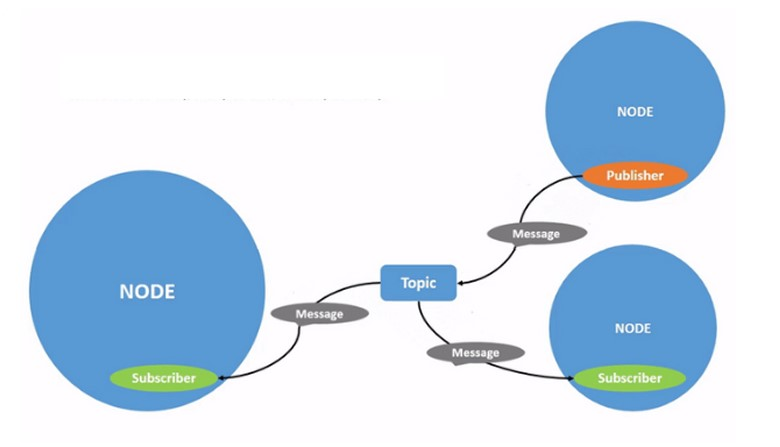
\includegraphics[width=\linewidth]{"images/nodi.jpg"}
\caption{Funzionamento protocollo pub/sub su ROS}
\label{fig:myImageLabel}
\end{figure}
\end{itemize}

\item \textbf{ROS message}:  I messaggi utilizzati in ROS sono strutture dati organizzate in campi, e per ciascun campo è specificato il tipo di dato che contiene. È possibile personalizzare i messaggi creando un file in cui si definiscono i campi necessari e salvandoli nel formato msg. ROS offre la possibilità non solo di definire nuovi tipi di messaggi, ma include anche una vasta libreria di messaggi predefiniti sviluppati dagli stessi creatori di  ROS, che coprono una vasta gamma di scenari. Questi tipi di messaggi personalizzati possono essere utilizzati non solo all’interno del nodo in cui sono stati definiti, ma anche in tutti i nodi in cui sono installate le dipendenze del nodo che utilizza quel messaggio.\\

\begin{figure}[t!]
\centering
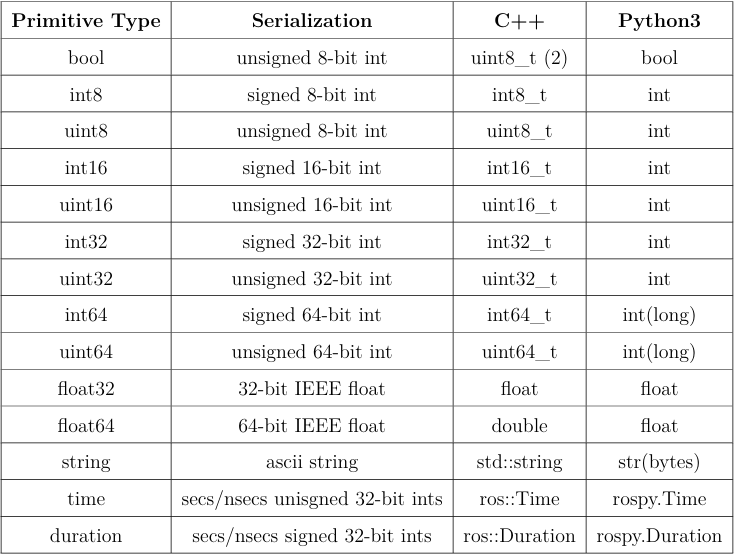
\includegraphics[width=\linewidth]{"images/tipi.png"}
\caption{Rappresentazione dei vari tipi su ROS}
\label{fig:myImageLabel}
\end{figure}
\end{enumerate}

Dopo aver introdotto la terminologia necessaria per riuscire a discutere di ROS
 in maniera appropriata, prendiamo in considerazione un nodo e andiamo a studiarne i
 componenti a livello implementativo.
\begin{lstlisting}[language=bash, caption={Creazione di un nodo ROS}]
$ source /opt/ros/foxy/setup.bash
$ ros2 pkg create -build-type ament_cmake <package_name>
\end{lstlisting}

Per ogni nodo sono presenti quattro directory principali oltre alla \textit{CMakeLists.txt} che rende la compilazione più snella da parte dell’utente e al \textit{package.xml} che definisce il pacchetto.
\begin{enumerate}
\item \textbf{config}: É presente un file di configurazione in cui possono essere definiti dei
 parametri statici che vengono poi recuperati dal nodo e utilizzati durante l’esecuzione. La comodità di utilizzare dei parametri di questo tipo è che non bisogna ricompilare il nodo se vengono modificati.
 
\begin{lstlisting}[language=bash, caption={Esempio di un file config}]
/package_name:
 	ros__parameters:
 	esempio_parametro: 1
 	general:
 	esempio_parametro: "prova"
\end{lstlisting}

\item \textbf{include/name\_node}: Si possono trovare tutti i file di intestazione che defini
scono le interfacce o le dichiarazioni delle classi, delle funzioni o delle variabili
 utilizzate all’interno del pacchetto. Questi file possono essere inclusi in altri file
 sorgente all’interno del pacchetto o in pacchetti esterni che desiderano utilizzare
 le funzionalità fornite dal pacchetto.
 
\item \textbf{launch}:  contengono i file che permettono al nodo di essere eseguito in maniera
 più snella e controllata. Per ogni file config che viene creato all’interno di un
 nodo è necessario aggiungere il percorso della directory in cui è presente il file di
 configurazione.
 
\begin{lstlisting}[language=bash, caption={Esempio di un file launch}]
def generate_launch_description() :
 	config_node = os.path.join
 	(
 	get_package_share_directory('package_name'),
'config',
'package_name_conf.yaml'

\end{lstlisting}
 \item \textbf{src}: Contiene il codice sorgente effettivo del pacchetto, inclusi i file sorgente per
 i nodi ROS2, le librerie personalizzate le classi e le funzioni che costituiscono il
 comportamento del pacchetto.
 
\end{enumerate}

L’ultima parte sulla visione iniziale di ROS2 è quella che riguarda la compilazione e
 l’installazione dei nodi all’interno del \textbf{ROS Environment}.
 
\begin{lstlisting}[language=bash, caption={ Compilazione di un pacchetto ROS e attivazione dell’Environment
}]
	$ colcon build --symlink-install
 --continue-on-error --package-select <package_name>
 
 # in questo modo posso eseguire file launch come se fossero nella cartella corrente
	$ source ./ros2_env/install/setup.bash
	$ ros2 launch package_name package_name_launch.py
\end{lstlisting}

